% Template for seminar reports
% Computer Vision Group, Visual Computing Institute, RWTH Aachen University
\documentclass[twoside,a4paper]{article}
\usepackage[utf8]{inputenc}
\usepackage{a4}
\usepackage{fancyhdr}   
%\usepackage{german}    % Uncomment this iff you're writing the report in German
\usepackage{makeidx}
\usepackage{color}
\usepackage{t1enc}		% German letters in the "\hyphenation" - command
\usepackage{latexsym}	% math symbols
\usepackage{amssymb}    % AMS symbol fonts for LaTeX.
\usepackage{graphicx}
\usepackage{pslatex}
\usepackage{ifthen}
\usepackage{booktabs}
\usepackage[T1]{fontenc}
\usepackage{pslatex}
\usepackage{psfrag}
\usepackage{subfigure}
\usepackage{url}
\usepackage{datetime}
\usepackage{xspace}
\usepackage{multirow}
\usepackage[bb=boondox]{mathalfa}
\usepackage{biblatex}
\addbibresource{abbrev.bib}
\usepackage{float}
\restylefloat{table}
\usepackage{hyperref} 
\usepackage{acronym}
\usepackage[symbols,nogroupskip,record]{glossaries-extra}
% \GlsXtrLoadResources[
%  src={symbols.bib},
%  type=symbols,% put these entries in the 'symbols' glossary
% ]


\newdateformat{monthyeardate}{\monthname[\THEMONTH] \THEYEAR}

% Do not change these sizes and do not add superfluous 
% pagebreaks to increase the page count.
\setlength{\oddsidemargin}{3.6pt}
\setlength{\evensidemargin}{22.6pt}
\setlength{\textwidth}{426.8pt}
\setlength{\textheight}{654.4pt}
\setlength{\headsep}{18pt}
\setlength{\headheight}{15pt}
\setlength{\topmargin}{-41.7pt}
\setlength{\topskip}{10pt}
\setlength{\footskip}{42pt}
\setlength{\parindent}{0pt}

\makeatletter
\DeclareRobustCommand\onedot{\futurelet\@let@token\@onedot}
\def\@onedot{\ifx\@let@token.\else.\null\fi\xspace}
\def\eg{\emph{e.g}\onedot} \def\Eg{\emph{E.g}\onedot}
\def\ie{\emph{i.e}\onedot} \def\Ie{\emph{I.e}\onedot}
\def\cf{\emph{c.f}\onedot} \def\Cf{\emph{C.f}\onedot}
\def\etc{\emph{etc}\onedot} \def\vs{\emph{vs}\onedot}
\def\wrt{w.r.t\onedot} \def\dof{d.o.f\onedot}
\def\etal{\emph{et al}\onedot}
\makeatother

% =========================================================================
\graphicspath{{pictures/}}
\setcounter{secnumdepth}{3}
\setcounter{tocdepth}{3}

% =========================================================================
\begin{document}
\begin{titlepage}
\begin{center}
\ 
\vspace{3.5cm}

\textsf{
RWTH Aachen University \\
Faculty of Mathematics, Computer Science and Natural Sciences\\
Media Informatics
}

\rule{\linewidth}{1pt}

\vspace{1.75cm}
\LARGE
\textbf{Master's Thesis}

\vspace{1.7cm}
\huge
Development of a Source Library for Transfer Learning: Leveraging Clustering and Contrastive Learning Techniques

\vspace{3.0cm}
\Large
Sneha Banerjee\\
\large
Matriculation Number: 430069

\vspace{0.5cm}
\today

\vspace{1.05cm}
\rule{\linewidth}{1pt}

\vspace{0.5cm}
\textsf{\textbf{
\normalsize
\begin{tabular}{ll}
Examiner: & Prof. Dr. Christian Bauckhage\\
Supervisor:  & Daniel Schiller\\
\end{tabular}
}}
\end{center}

\end{titlepage}


\begin{titlepage}

\Large\textbf{Declaration of Originality}
\paragraph{}
\hskip-0.8cm
    \begin{tabular}{p{1.8in}p{4.8in}}
        Name & Sneha Banerjee \\
        Matriculation number & 430069 \\
        Address & Allmandring 8A,70569 Stuttgart \\        
        Title & \textit{Development of a Source Library for Transfer Learning: Leveraging Clustering and Contrastive Learning Techniques} \\
    \end{tabular}

\vspace{1cm}
I now declare,
\begin{itemize}
    \item that I wrote this work independently,
    \item that no sources other than those stated are used and that all statements taken from
other works—directly or figuratively—are marked as such,
    \item that the work submitted was not the subject of any other examination procedure,
either in its entirety or in substantial parts,
    \item that I have not published the work in whole or in part, and
    \item that my work does not violate any rights of third parties and that I exempt the
University against any claims of third parties.
    \end{itemize} 
\end{titlepage}
\begin{abstract}
% +++++++++++++++++++++++++
% Insert your Abstract here (one paragraph summary)
 
% +++++++++++++++++++++++++
\end{abstract}

\tableofcontents
% =========================================================================

% +++++++++++++++++++++++++
% Insert your Text here
% +++++++++++++++++++++++++

\section{Introduction}
\pagenumbering{arabic}
\subsection{Motivation}
\subsection{Task and Goal}
\subsection{Approach}
\subsection{Contribution}


\section{Related Work}

\section{Background}
\subsection{Bin Picking}
\subsubsection{Definition and Application}
\subsubsection{Gripper Types}
\subsubsection{Model-Based Approaches}
\subsubsection{Model-Free Approaches}
\subsubsection{Robot System}
\subsection{Deep learning-based 3D Image processing}
\subsubsection{Convolution Neural Network}
Inspired from the visual cortex of humans, convolutional neural network(\ac{CNN} or ConvNet) is a type of deep neural network designed for processing data which appear in a grid like manner like images, videos, etc.  It was introduced by Yann LeCun et. al in \cite{lecun1998gradient} in 1998.  It gets it name because of the usage of a special kind of linear mathematical operation called the convolution instead of using matrix multiplication as prevalent in the pre-existing neural networks. The key components of a \ac{CNN} are - Convolution layer, activation function, pooling layer, loss function, output layer. The principle building block if a CNN is the convolution layer. It consists of a number of learnable filters (kernels) which can be visualised like a cubic block. The success of \ac{CNN}s can be attributed to three major concepts: sparse interactions, parameter sharing and equivariant representations.
\paragraph{Sparse interactions}
In traditional fully connected network, matrix multiplication is performed which involves a parameter matrix. The interaction between input and output units are captured by a distinct parameter in the parameter matrix. But \ac{CNN}s have {sparse interactions, i.e. only a subset of units or neurons in a layer is connected to a local region in the preceding layer. This is done by using kernels that are significantly smaller than the input. This implies, less number of parameters need to be stored which reduces the memory consumption and also it is computationally efficient because it has to perform fewer operations. For example, if there are m inputs and n outputs, the fully connected network would need to store \textit{m} x \textit{n} parameters and have a runtime of \textit{O}(\textit{m} x \textit{n}) time complexity per input. On the other hand, if we restrict the number of connections for each unit to be k, then we would have \textit{k} x \textit{n} and have a runtime of \textit{O}(\textit{k} x \textit{n}) time complexity per input, where k is quite some fold lesser in magnitude as compared to m. Moreover, since convolution layers are stacked upon one another in a deep convolution network, units in the deeper layers have a larger receptive field, because of it's indirect interaction with a larger region in the input.
\paragraph{Parameter sharing}
Another important focus behind using the convolution layer was to reduce the number of parameters in a \ac{FCN}. For example in a 1024*1024 image, a \ac{FCN} would have over 1 million hidden units, which means it would have over 1 trillion trainable parameters. But the pixels in an image are only locally correlated. So, \ac{CNN}s make use of the kernels to limit the focus on smaller regions on the image at a time known as the receptive field. This significantly reduces the number of trainable parameters, thus reducing the memory consumption. \cite{ConvNet}.    These layers perform a convolution operation between the input (eg. image) \textit{I} and the kernel \textit{K} to produce an output \textit{S} known as the feature map as in Eq.\ref{eq:conv}.
\paragraph{Equivariant Representations} 
A function is said to be equivariant if the input to a function is changed, then the output changes in the similar way. Because of the parameter sharing mechanism, convolutions operations are translation equivariant. When the kernels the applied on an input image, the convolution layers generate a 2D map of where the particular feature occurs in the particular image. Furthermore, a pixel is related to it's neighboring pixels to form a meaningful context(create a feature e.g. an edge in an image) but it is not limited to where it can occur throughout the image. Thus it creates multiple filters each of which look for the same feature throughout the image. But it is also to be kept in mind that convolution is not equivariant to other geometric and affine transformations like rotation, scaling, etc. 
 Since convolution operations are commutative in nature, Eq. \ref{eq:conv} can also be written as Eq.\ref{eq:conv_com}. Typically, Eq. \ref{eq:conv_com} is easier to incorporate into a machine learning library since values for both 'm' and 'n' varies within a small range.\cite{Goodfellow-et-al-2016}
\begin{equation}
    \label{eq:conv}
    \mathit{S(i,j)}= \mathit{(I*K)(i,j)} = \sum_{m}\sum_{n}\mathit{I(m,n)K(i-m,j-n)}
\end{equation}
\begin{equation}
    \label{eq:conv_com}
    \mathit{S(i,j)}= \mathit{(I*K)(i,j)} = \sum_{m}\sum_{n}\mathit{I(i-m,j-n)K(m,n)}
\end{equation}
\paragraph{Activation function}
The next step in a \ac{CNN} is to apply an activation function. the purpose of using a non linear activation function is to capture the non-linearity in the data. Moreover if non-linearity is not used in between the multiple layers of a neural network, the network is effectively only one layer deep which is not capable even to capture the non-linearity in real world datasets. \ac{ReLU} is the most commonly used non-linear activation function used in \ac{CNN}s because unlike sigmoid function or tanh function it does not penalise "too correct" data points. Another remarkable benefit of using \ac{ReLU} is it's ability to propagate gradient through deep networks with a constant factor. Also it is more memory efficient to use \ac{ReLU} as it doesn't require to store the \ac{ReLU} outputs separately as compared to tanh outputs.
\paragraph{Pooling}
The third step of a \ac{CNN} is to use the pooling layer. The main purpose of this operation is to make the detection of the features robust to the exact location of the eye (i.e. invariant to small translations). The different types of pooling operations are - max pooling and average pooling. It also helps in reducing the dimensionality of the input without losing too much information. This is done to make the computations faster down the deeper layers of the network. If the pooling operations are performed after every k pixels, then the next layer processes inputs that are k times lesser. Since the number of parameters in a layer are dependent on the size of the input to the layer, it significantly reduces the computational overhead on using pooling operations. 

\subsubsection{Clustering Algorithms}
When the dataset does not have any labelled data, then it is said to be unsupervised learning. In this case, there is no ground truth available to measure the correctness of the outputs generated by the \ac{ML} models. The primary focus of unsupervised learning is to find hidden and interesting pattern in the data. Unsupervised learning is of utmost importance in the \ac{AI} world as several real world datasets do not have available annotations, which requires a lot of human effort. Unsupervised learning algortihms can be broadly categorized into the following domains-clustering, dimensionality reduction, and association analysis. Clustering algorithms aim at grouping unlabelled data into groups or clusters based on how similar or dissimilar the datapoints are to one another. It can reveil underlaying hidden pattern in the data and is used in applications like image segmentation, fraud detection, etc. Dimensionality reduction is reduces the number of irrelavant features or dimensions of the dataset. The inclusion of more features does help in the better representation of the dataset but it also significantly increases the memory consumption and complexity to work with it. Also it is often difficult to visualise real-life datasets with too many features. Association analysisis a rule-based unsupervised learning method that reveals the relationship between attributes in the dataset. It is used in applications like market analysis, intrusion detection, etc.\\
Clustering algorithms can be broadly classified into the following categories: density-based, distribution-based, and hierarchical-based. In density-based clustering, the algorithm looks for areas of high concentration of the datapoints and groups them as a cluster. The benefit of this algorithm is that the shape a cluster can be is not limited and hence doesn't necessarily have to be convex in nature as show in Fig. \ref*{fig:dbscan}.
\begin{figure}[t]
    \centering
    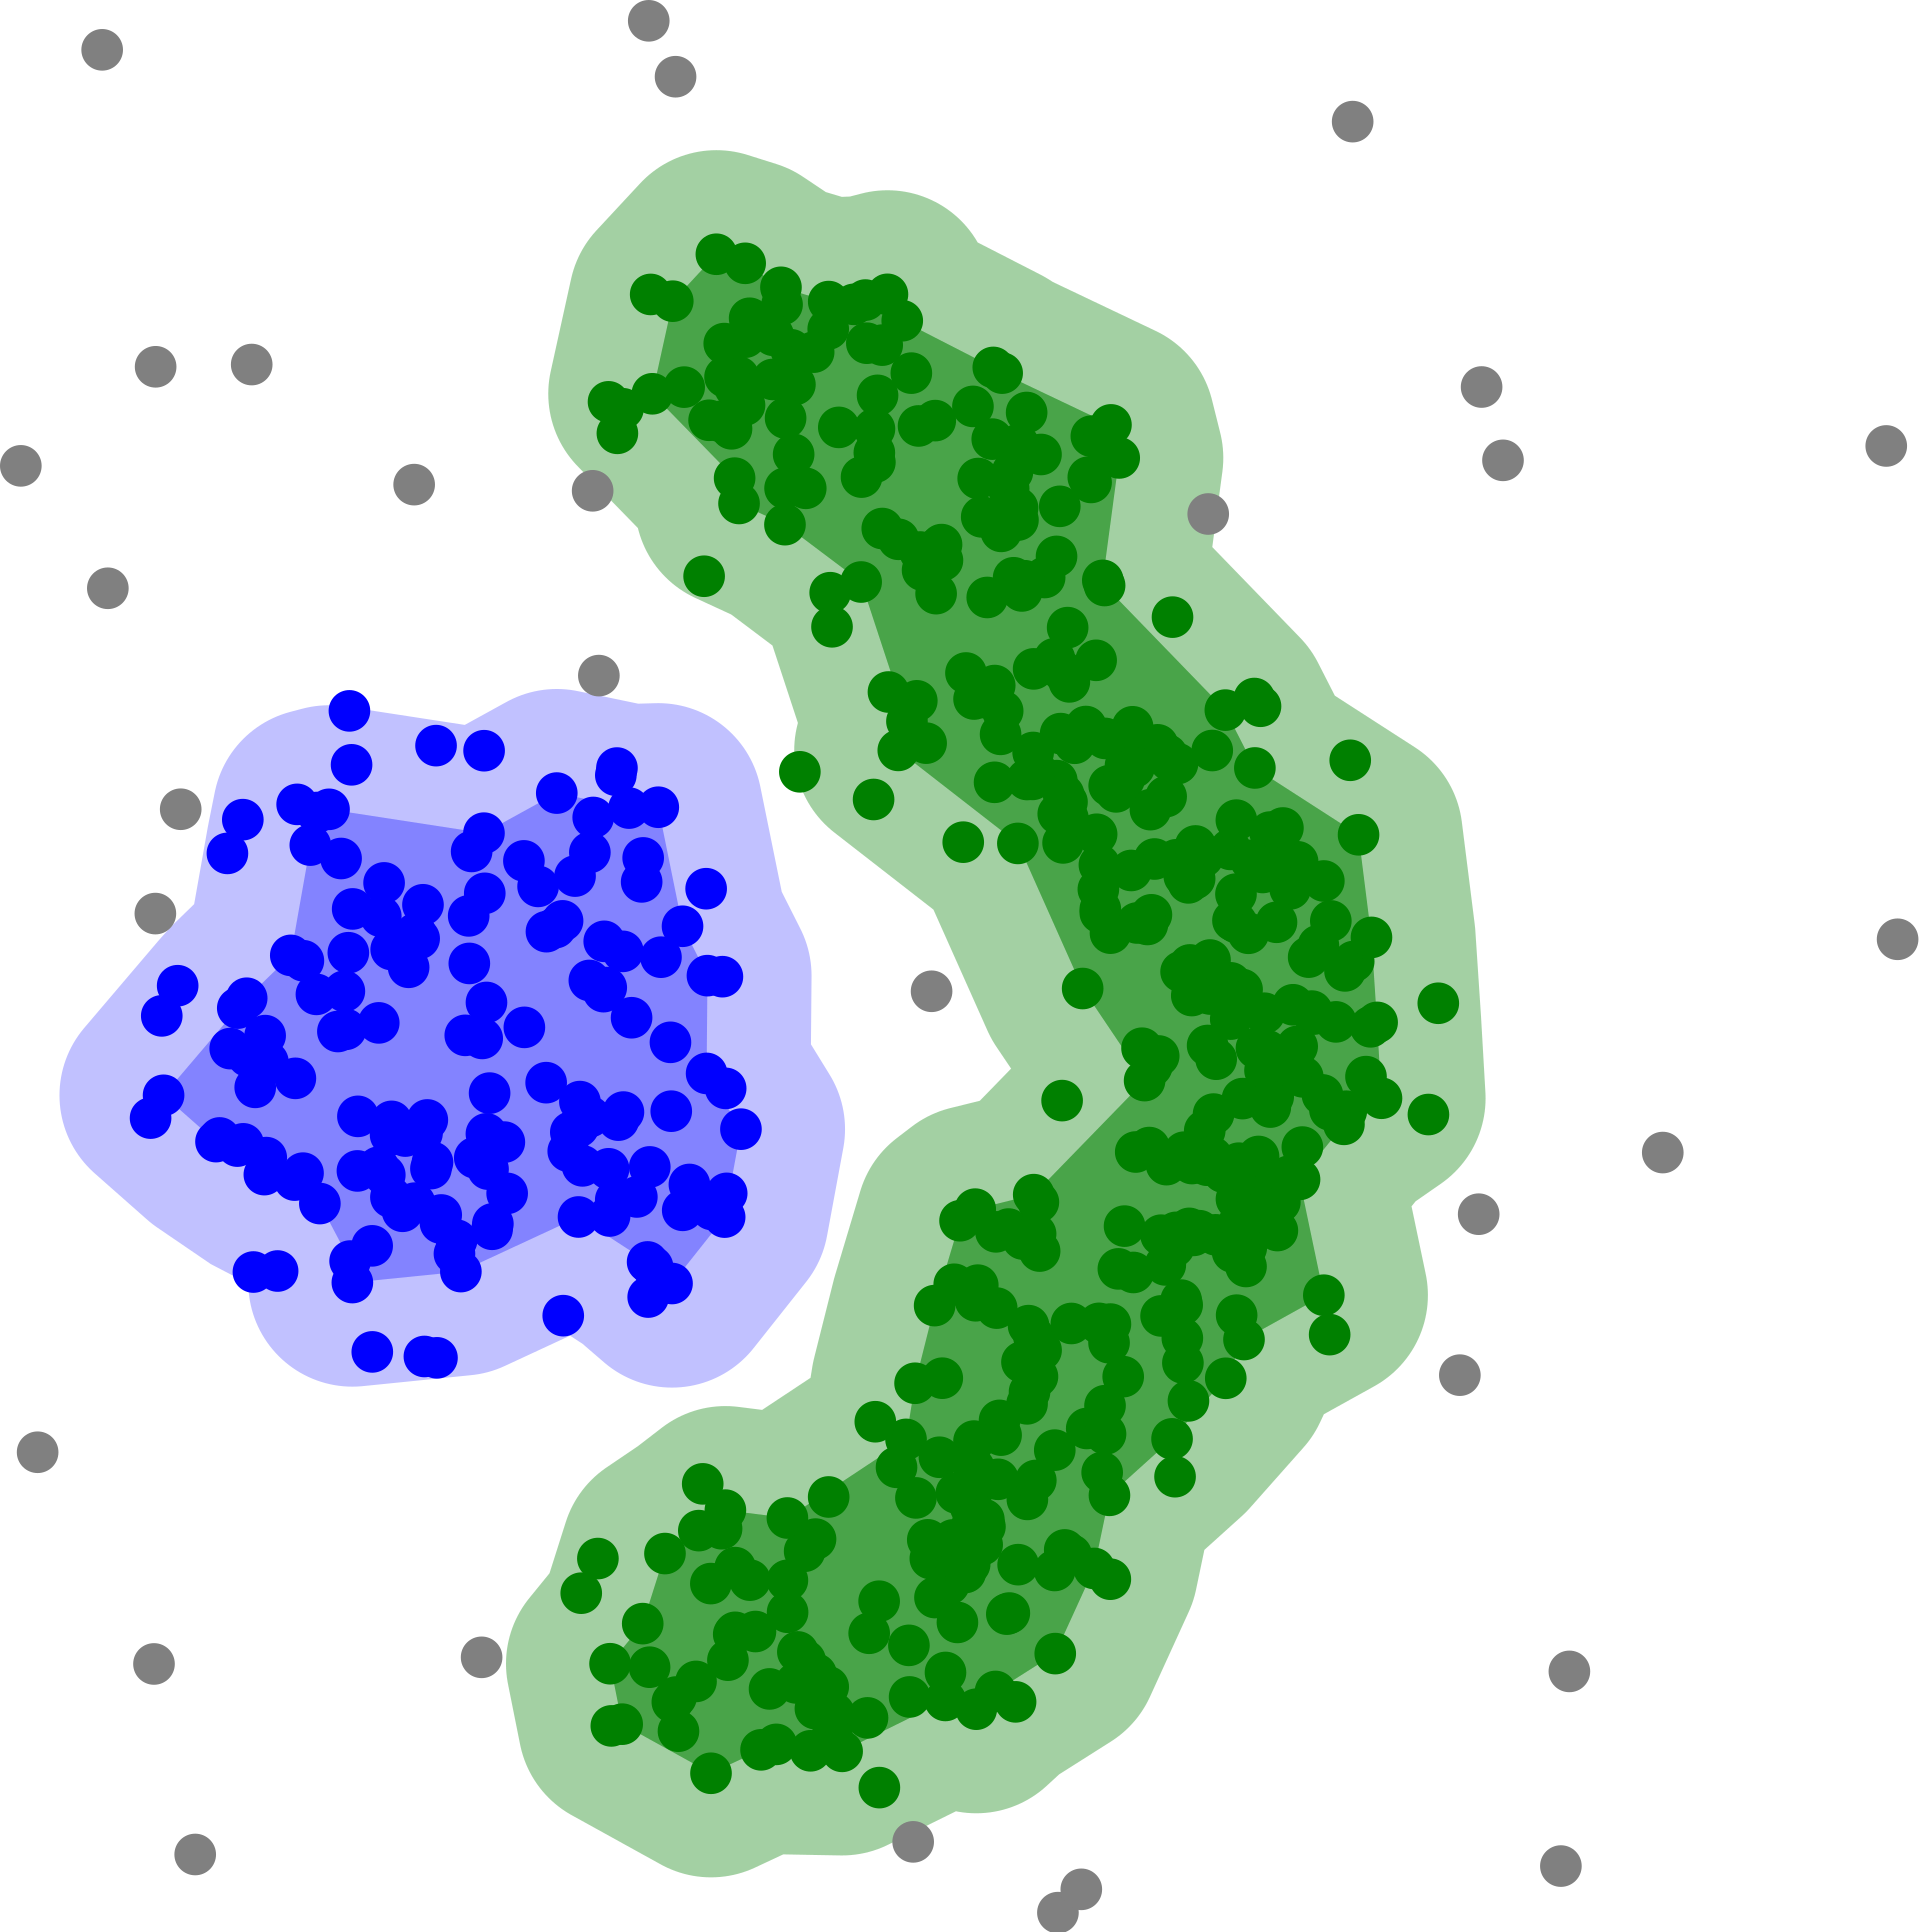
\includegraphics[width=200pt,height=150pt]{pictures/DBSCAN-density-data.png}
    \caption{\ac{DBSCAN} can find non-linearly separable non-convex clusters.\cite{dbscanWiki}}
    \label{fig:dbscan}
\end{figure} 
Moreover, these algorithms are also very robust to outliers as they do not force the outliers to belong to any category but are rather ignored as it is unlikely that outliers can form an area of high concentration of datapoints. I have carried on the experiments on this thesis on two such density-based clustering algortihms called \ac{DBSCAN}\cite*{dbscan} and \ac{HDBSCAN} algorithms\cite*{hdbscan}. The available scikit-learn implementations were used for this purpose\cite*{scikit-learn}. The \ac{DBSCAN}\cite*{dbscan} algortihm  does not require the users to define the number of clusters to be generated which doesn't force dissimilar datapoints to belong to the same cluster. However, this algorithm was still sensitive to two parameters $\epsilon$, the maximum distance betwwen the datapoints to be considered in the same cluster and the minimum number of samples in the cluster which the user needs to define \cite*{scikit-learn}. But finding an optimum value for these parameters often require domain expertise and are dependent on the data. The \ac{HDBSCAN}\cite*{hdbscan} algorithm mitigates this issue and thus does not require the user to define these two parameters. It is a hierarchical density-based clustering that performs the \ac{DBSCAN} algorithm over multiple $\epsilon$ values to find the most stable result. In distribution-based algorithms, a datapoint is said to be a member of the cluster depending on the probability of it's membership to the cluster. The more the distance of a point increases from the centre of the cluster, the less is it's probability of belonging to that cluster. Centroid-based algorithms groups the datapoints based on some initial cluster centres. Once all the dataspoints are softly assigned to some cluster membership, the cluster centres are recalculated and this process is iterated until convergence. These algorithms are sensitive to the initial parameters like the cluster centres chosen in the first step. Another major disadvantage of these clustering algorithms are that they always form spherical clusters. The user also needs to define the number of clusters the dataset is to be grouped in, which makes it sensitive to outliers. However, these algorithms can be executed very fast and we have used two such algorithms in our experiments- K-Means\cite*{kmeans}and K-Medoids\cite*{kmedoids}. In K-Means, the mean of the datapoints of the clusters is assigned as the cluster-centroid. It might not be an actual datapoint in the dataset, rather a blurred, noisy average of a datapoints in the cluster. On the contrary, the K-Medoids algortihm assigns an actual datapoint of the dataset, that is most centrally located as the cluster centroid as shown in Fig.\ref*{fig:kmean-kmedoid}. Thus K-Medoids is more robust to outliers and noises as compared to K-Means.
\begin{figure}[h]
    \centering
    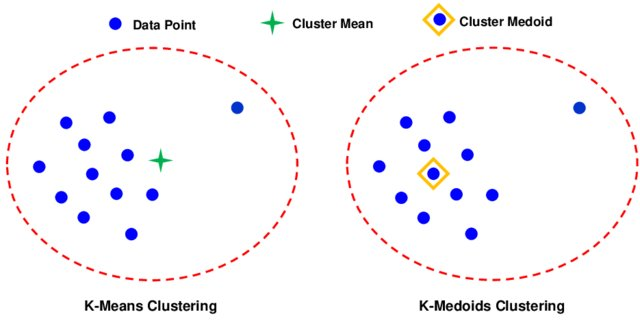
\includegraphics[width=200pt,height=150pt]{pictures/The-graphical-representation-of-the-difference-between-the-k-means-and-k-medoids_W640.jpg}
    \caption{Difference between K-Means and K-Medoids.\cite{kmean-kmedoid}}
    \label{fig:kmean-kmedoid}
\end{figure}
Hierarchical-based clustering algorithm that form a hierarchy of clusters. Datapoints in a cluster are more similar to each other as compared to other groups. this hierarchy of clusters is visualised by a hierarchy tree called dendograms. hierarchical clustering algorithms can be of two types - agglomerative and divisive. In agglomerative clustering, each datapointis considered as a separate cluster in the first step. Then these clusters are merged into one another until only one cluster remains. Thus at the end, the last level cluster consists of all teh datapoints in the dataset. The divisive method is the reverse procedure of the aggomerative method. In the beginning, all the datapoints are considered to be in a single cluster and gradually the cluster is broken into smaller clusters, untill each cluster consists of only one datapoint. A visual representation of a dendogram has been shown in Fig.\ref*{fig:dendogram}
\begin{figure}[t]
    \centering
    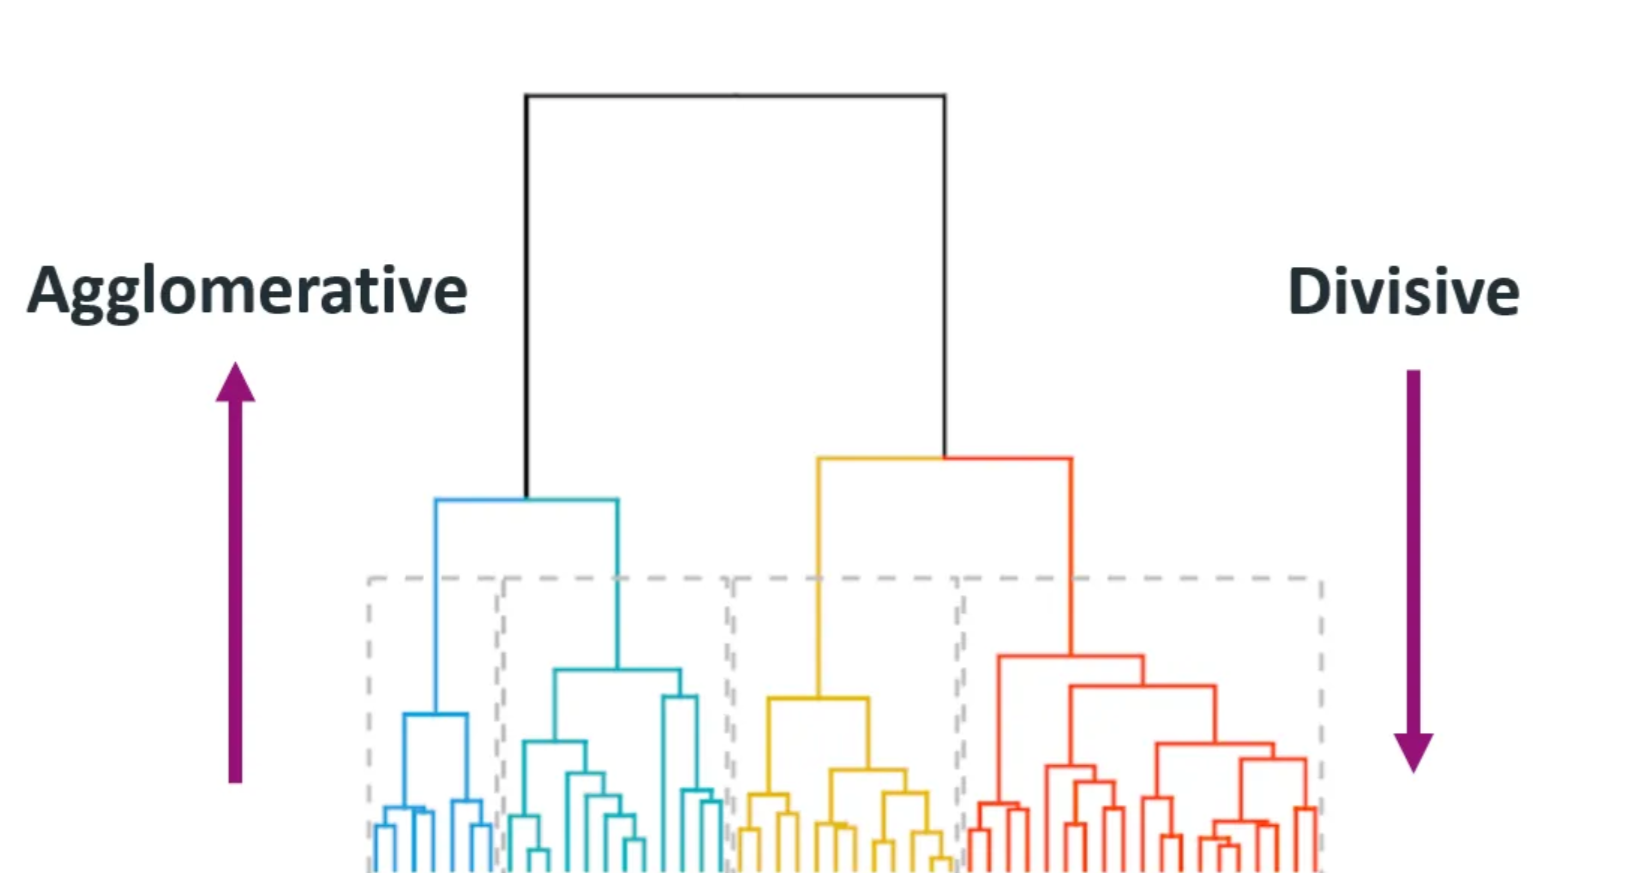
\includegraphics[width=200pt,height=150pt]{pictures/dendogram.png}
    \caption{A dendogram in hierarchical clustering.\cite{dendogram}}
    \label{fig:dendogram}
\end{figure}

\subsubsection{Autoencoders}
\subsubsection{Siamese Network}
\subsubsection{YOLO}
\subsection{Transfer learning}
\subsubsection{Definition}
\subsubsection{Categories}
\subsubsection{Relevant Algorithms}
\subsection{Network generation process with PQ-Net++}



\section{Method}
\subsection{Suitable Algorithm and Adjustments}
\subsection{Whatever new Concept we propose}
\subsection{Architecture}
\subsection{Source and Target Objects}
\subsection{Data Generation}
\subsection{Important Aspects}

\section{Application of algorithms}

\section{Experiments}

\section{Implementation in a Bin Picking Cell}

\section{Conclusions}
\subsection{Discussions}
\subsection{Limitations}
\subsection{Future Scope}

\section{Summary}

\section*{List of Acronyms}
\addcontentsline{toc}{section}{List of Acronyms}

\begin{acronym}
    \acro{CNN}{Convolutional Neural Network}
    \acro{FCN}{Fully Connected Network}
    \acro{ReLU}{Rectified Linear Unit}
    \acro{ML}{Machine Learning}
    \acro{AI}{Artificial Intelligence}
    \acro{DBSCAN}{Density-Based Spatial Clustering of Applications with Noise}
    \acro{HDBSCAN}{Hierarchical Density-Based Spatial Clustering of Applications with Noise}
\end{acronym}
\addcontentsline{toc}{section}{List of Figures}
\listoffigures
\addcontentsline{toc}{section}{List of Tables}
\listoftables
\section*{List of Symbols}
\addcontentsline{toc}{section}{List of Symbols}


% \printunsrtglossary[type=symbols,style=long,title={List of Symbols}]


% =========================================================================
\printbibliography[heading=bibintoc,title={Bibliography}]
\end{document}
